The use of scintillators in radiation detection is one of the most used technics in nuclear physics. The scintillator is a material that is able to convert the kinetic energy of the incoming particles in light (photons in the visible energy range) which we can detect and quantify. It happens because the radiation excites and ionizes the scintillating atoms which, after that, are immediately de-exciting (with times of the order of picoseconds), emitting photons.

This conversion should be linear in a wide energy range of incoming particles and it is necessary that this material has good optical properties, such as being transparent to the wavelenght of their own emission and having a refractive index as close as possible to the glass for optimizing optical coupling with photosensors.

The photon emission in the scintillator is a stadistical process, which means that two exactly the same events will emmit different number of photons. It follow a poisson statistics so when we speak about the number of emmited photons we speak about the mean number of photons.

There are two types of scintillators, organics and inorganics. Inorganic scintillators normally have a higher atomic number and density so their light output are higher. Due to these reasons they are better for gamma-ray spectroscopy (take into account figure \ref{ProcessesPhotons}). Organic scintillators generally are faster and they are commonly used for beta spectroscopy and neutron detection. In this seccion I focus my explanation mainly on organic scintillators since they are the ones we have used in our research. 

Organic scintillators are based on a scintillator material, which produces light, dissolved in a base solvent. This solvent is normally based on aromatic hydrocarbons (carbon atoms linked together), that is, they are mainly composed of carbon and hydrogen atoms as we can see in the molecules of some of the most widely used scintillators, $\ce{C_{18}H_{14}}$, $\ce{C_{24}H_{22}N_{2}O}$ or $\ce{C_{15}H_{11}NO}$ whose average atomic numbers are between 3,5 and 5.

The scintillator molecules, in which the organic scintillators are based, have the so called $\pi$-electron structure. The energy levels of their electrons are commonly ilustrated with a Jablonsky diagram, figure \ref{JablonskyDiagram}, where we can see the fundamental single state, $S_{0i}$, where the valence electrons are, the excited single states, $S_{jk}$, and the excited triple states, $T_{lm}$. De energy difference between $S_1$ and $S_0$ states is around $3$ or $4~\eV$, energy range of the visible photons. We can see in this diagram that each of this energy states are subdivided in smaller energetic sublevels whose distance between them are around $0.15~\eV$. This finer energy structure is due to the excitations of molecular vibrational modes and they are expresed with the second index of the energy states.

\begin{figure}[htbp]
\centering
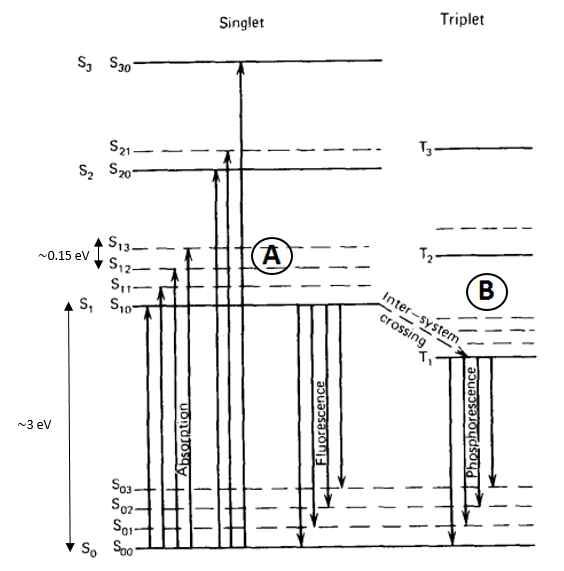
\includegraphics[scale=0.6]{3DesignPrinciples/JablonskyDiagram.png}
\caption{Jablonsky diagram.\label{JablonskyDiagram}~\cite{Knoll}}
\end{figure}

Because of the reason that the distance between all energy levels and sublevels are larger than the termal energy, $0.025~\eV$, non-exciting electrons are in the lowest state $S_{00}$ at standar temperature conditions.

When a particle deposits their kinetic energy on a scintillator, their valence electrons are exited to higher single energetic states very fast (times of the order of picoseconds) which is expressed with upwards direction arrows in the figure \ref{JablonskyDiagram} and they are quickly de-excited to the first single excited state, $S_{10}$, through non-radiactive processes known as internal conversion.

Now, this electrons can de-excited to the fundamental single state, $S_{00}$, through three different physical mechanisms:

\begin{itemize}

\item{} The prompt fluorescence(process A in figure \ref{JablonskyDiagram}), where the electron in the $S_{10}$ energy level  is de-excited to some sublevel of the fundamental state $S_{0i}$, emitting a photon with an energy equal to the energy difference of these levels (around $3~\eV$, visible light). This process happens immediately after the excitation of the scintillator molecules (around tens of nanoseconds after excitation). Each scintillator has a characteristic emission spectrum that defines its response due to the fluorescence mechanism. 

Now we can understand why organic scintillators are practically transparent to their own fluorescense emission. This is because of the reason that there existe a quenching effect in each de-excitation process whereby there are a lost of radiated energy. Due to that, all emmited  photons by the scintillator have less energy than the required energy for excitation. This effect is called Stokes shift and it's represented with a general wavelenght spectrum in the figure \ref{StokesShift}.

\begin{figure}[htbp]
\centering
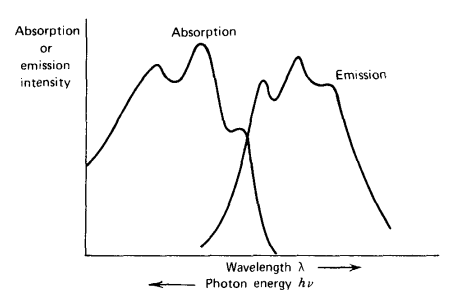
\includegraphics[scale=0.7]{3DesignPrinciples/StokesShift.png}
\caption{Stokes shift.\label{StokesShift}~\cite{Knoll}}
\end{figure}

One of the most important parameters in nuclear physics is the scintillation yield, whcih is the fraction of particle energy that is converted in light. All mechanisms which don't produce prompt fluorescence, like phosphorescence or delay fluorescence, which we will see later, or even internal conversion, contribute to reduce this parameter. The signal of the scintillator depends on the type of particle so, the scintillation yield will be different. This factor is normally given by the manufacturer for mips (minimum ionized particles, that's, for example, electrons with $500~\keV$ or more) in number of photons per $\MeV$.

The intensity of the fluorescence emission in an organic scintillator during time is a combination of two exponential functions, one associated with the lifetime of the level, $\tau$ (on the order of nanoseconds), and the other associated with the energetic level population, $\tau_1$ (on the order of picoseconds).

$$I=I_0\left(e^{t/\tau} - e^{t/\tau_1}\right) \cite{Knoll}$$

\item{} The phosphorescence, where the electron, which is in the first single excited state, cross to a triple excited state (process B in figure \ref{JablonskyDiagram}) with a process called "intersystem crossing". This is a metastable state with a much longer lifestime so electrons in this state are de-excited to the $S_{0i}$ state, emitting a photon much later than phosphorescence. This process can happen up to $10^{-3}$ seconds after scintillator excitation.

\item{} Delayed fluorescence, which occurs when an electron is in a triple excited state but whose transition to the ground state is forbidden. In this case, this electron can interact with another in the same state and return to the first single state ($S_{1}$ is more energetic level than $T_{1}$) and quickly de-excited to the ground state. 

$$T_{1} ~+~ T_{1}~ \longrightarrow ~ S_{1} ~+~ S_{0} ~+~ phonons$$

This emission has the same emission spectrum as immediate fluorescence, but occurs later.

\end{itemize}

The scintillating detectors generally use the prompt fluorescence light as output signal so a good scintillator should increase it and reduce other possible physical mechanisms.